\chapter{Introduction}
\label{chap:introduction}

Rise of cheap cloud storage solutions has encouraged users as well as enterprises to
resort to commercial cloud storage services such as Google Drive \cite{googleDrive} and 
Dropbox \cite{dropbox}. This has in turn triggered a large influx of data to be stored
in remote servers. In order to keep the prices competitive, service providers require
space saving techniques that can be deployed on a large scale without sacrificing
response time and reliability. In this setting, deduplication plays an important role \cite{practicaldedup}.
Deduplication is a well known technique that enables storage providers to store a single
copy of the data regardless of how many clients has uploaded the same data.
\\ \\
To see how a typical deduplication scheme works, imagine Alice uploads a file
$M$ to the server. Bob then requests to upload his copy of the same file $M$. The server identifies
that $M$ is already stored and simply updates the metadata associated with $M$ to show
that the file is owned by both Alice and Bob.
\\ \\
Based on the granularity of deduplication, two different flavours exist:
\begin{enumerate}
	\item \textit{File-level deduplication}: In this level, deduplication is
	exploited on the file level. Entire files are compared for deduplication
	which means only a single copy of each file will be stored.
	
	\item \textit{Block-level deduplication}: The files are divided into blocks and
	each block is checked for redundancy. This is more fine-grained and has its own
	advantages and disadvantages.
\end{enumerate}

Based on the deduplication architecture, there are two different strategies:
\begin{enumerate}
	\item \textit{Server-side deduplication}: Here the clients are oblivious to any of the
	underlying deduplication techniques. The file is uploaded to the server which
	may perform deduplication techniques. As far as the client is concerned, the upload and download
	functionalities work the same. This technique is also referred to as 
	\textit{target-based deduplication}
	
	\item \textit{Client-side deduplication}: In this technique, the client sends a \textit{tag}
	to the server before uploading the file. The \textit{tag} serves as a unique identifier of
	the entire data (e.g., a hash value) and is much shorter than the file. The server checks for
	redundancy and if a match occurs, the file is not sent over the network. Client-side also called
	\textit{source-based deduplication}, has the added advantage of saving network bandwidth.
\end{enumerate}
Deduplication along with privacy is a conflicting idea. On one hand, users will want
their data to be encrypted for a variety of reasons including personal privacy, corporate policy or
even legal reasons. On the other hand, 
the cloud providers would like to save space by identifying the file uploaded by 
the user and storing a single copy of the file.
Secure deduplication aims to resolve this conflict.	

\section{Motivation}
File level deduplication achieves significant space savings - as much as 75\% to 87\% depending 
on the file type \cite{practicaldedup}. Using deduplication,
cloud storage providers can save storage and thereby money which can in turn be transferred to
users in the form of cheaper storage options. By making deduplication compatible with privacy,
this can be achieved without the users having to sacrifice privacy.
\\ \\
Most of the existing deduplication schemes enables deduplication when files are identical. There
are several use cases when the files uploaded will be very close to each other. For instance, 
when a user uploads several photos which are taken quickly one after the other, the files
will be very close to one another. In this
paper, we put forward a scheme that can achieve deduplication across files. In this case, if a user
uploads a file to the server and a file that is close to this already exists in the server,
then the server will not store the entire file but a small piece (a $\Delta$) 
using which the original can be recovered later.


\section{Our Work}
\label{sec:intro}
This paper puts forward a scheme called $\scheme$ (deduplication across files) which enables deduplication even for files that are close to
each other. The basic idea is to divide the message space into several balls of same radius $\tau$
each with a message $\psi$. We use the hamming distance metric to do this. To encrypt a 
message $m$, it first is mapped to the corresponding $\psi$ that it belongs to. This $\psi$ is then
encrypted ($C_\psi$) and then uploaded along with a $\Delta$. $\Delta$ combined with $\psi$ will give
back the original message $m$. As long as the distance $\tau$ is small and the original
message has high enough entrpy, the $\Delta$ leaked will not compromise the security of the
encryption.\\ \\
To see that this enables deduplication, consider Figure \ref{fig:example}. Suppose Alice has
message $w_1$ that needs to be saved in the server. This will be uploaded to the server 
as encryption of $\psi$ ($C_\psi$) and $\Delta_1$. Later, Bob wants to upload $w_2$ and this
will be uploaded as $C_\psi$ and $\Delta_2$. The server needs to store only $\Delta_2$. Of course,
if Bob were also to upload $w_1$, deduplication is still achieved.

\begin{figure}[H]
	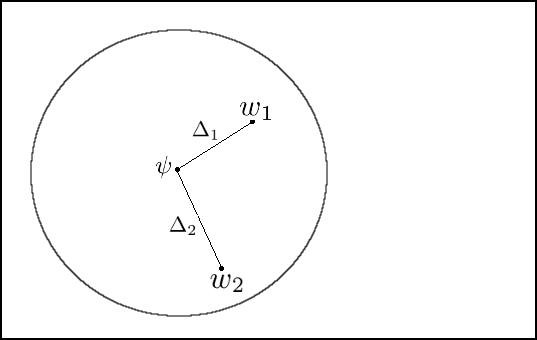
\includegraphics[scale=0.5]{example.png}
	\caption{Rectangle box represents the entire message space. Only one of many balls is shown}
	\label{fig:example}
\end{figure}



The rest of the paper is organised as follows: Section \ref{prelim} discusses the preliminaries needed 
and the ingredients that are used in this paper. Section \ref{sec:imle} explains Interactive MLE scheme
introduced in \cite{imle}, the adversarial model and the security game used. The construction of $\scheme$
is explained in section \ref{sec:constr} and its security is proved in section \ref{sec:res}.